\documentclass[a4paper, oneside, final]{scrartcl}
\usepackage{scrpage2} % Provides headers and footers configuration
\usepackage{titlesec} % Allows creating custom \section's
\usepackage{marvosym} % Allows the use of symbols
\usepackage{tabularx,colortbl} % Advanced table configurations
\usepackage{fontspec} % Allows font customization
\usepackage{color}
\usepackage[usenames,dvipsnames]{xcolor}

\usepackage{polyglossia}
\setmainlanguage{russian} 
\setotherlanguage{english}
\newfontfamily\russianfont[Script=Cyrillic]{Tahoma}

\defaultfontfeatures{Mapping=tex-text}
\titleformat{name=\section}[block]
  {\large\scshape\raggedright}
  {}
  {0pt}
  {\colorsection}
  [\titlerule]
\titlespacing*{\section}{0pt}{\baselineskip}{\baselineskip}

\newcommand{\colorsection}[1]{%
  \colorbox{LimeGreen!30}{\parbox{\dimexpr\textwidth-2\fboxsep}{#1}}}

\pagestyle{scrheadings} % Print the headers and footers on all pages
\addtolength{\voffset}{-2.3cm} % Adjust the vertical offset - less whitespace at the top of the page
\addtolength{\textheight}{5.7cm} % Adjust the text height - less whitespace at the bottom of the page

% FOOTER SECTION
%----------------------------------------------------------------------------------------

\renewcommand{\headfont}{\normalfont\rmfamily\scshape} % Font settings for footer

\cofoot{
\addfontfeature{LetterSpace=10.0}\fontsize{12.5}{12}\selectfont % Letter spacing and font size
{\Letter} kseniya.terekhina@phystech.edu  \ {\Large\Telefon} (916) 467-78-86 % Your email address and phone number % TODO: fake number
}
\newcommand{\tabitem}{{\textbullet}~}

\usepackage{graphicx}
\graphicspath{ {/} }
%----------------------------------------------------------------------------------------

\begin{document}

\begin{center} % Center everything in the document

% HEADER SECTION
%----------------------------------------------------------------------------------------

\begin{tabularx}{0.99\linewidth}{m{11.5cm}m{3cm}}

{\addfontfeature{LetterSpace=5.0}\fontsize{24}{24}\selectfont\scshape Ксения Терехина} & % Your name at the top 
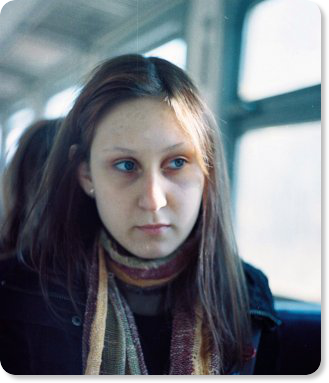
\includegraphics[height=3cm]{ksu-av.png} \\
\end{tabularx}

\section{\textbf{Образoвание}}

\begin{tabularx}{0.99\linewidth}{p{2cm}p{11.8cm}}
\multicolumn{2}{l}{\textbf{Московский физико-технический институт (МФТИ ГУ)}} \\
 2014 - 2016 &  {Магистр. Cистемный анализ и управление в больших системах} \\
 2010 - 2014 &  {Бакалавр. Cистемный анализ и управление} \\
 & ~ \\
\multicolumn{2}{p{1\linewidth}}{\textbf{Российская академия народного хозяйства и государственной службы \newline при Президенте РФ (РАНХиГС)}} \\
 2014 - 2016 &  {Магистр. Финансы и Экономика} \\
 2010 - 2014 &  {Бакалавр. Экономика} 
\end{tabularx}

\section{\textbf{Опыт работы}}
\begin{tabularx}{0.99\linewidth}{p{2cm}p{11.8cm}}

\multicolumn{2}{l}{\textbf{Институт прикладных экономических исследований при РАНХиГС}} \\
2014 - н/вр \rule{1.9cm}{.1pt} 1 год \newline 4 месяца & 
    \textbf{Младший научный сотрудник} \newline
\textbullet~ Построение экономических моделей с использованием метода групового учета аргументов (GMDH) \newline
\textbullet~Вейвлет анализ для исследования периодичности покупок железнодорожных билетов \newline
\textbullet~ Работа в среде Matlab и GMDH Shell\\
\end{tabularx}

\section{\textbf{Навыки}}
\begin{tabularx}{0.99\linewidth}{ p{5cm} p{8.8cm} }
Языки & Английский (Технический), Испанский (Базовый)\\
Языки программирования & Python, Matlab, Wolfram Mathematica, OxMetrics \\
Статистические пакеты  & Stata, Eviews \\
Прикладные программы & MS Office, OS Linux, Git, Vim, LaTeX \\
\end{tabularx}

\section{\textbf{Участие в конференциях}}
\begin{minipage}{.99\linewidth}
\textbullet~ INFOS2014, Польша, Сентябрь 2014\newline 
\textbullet~ 57-я научная конференция МФТИ, Москва, Ноябрь 2014 \newline
\textbullet~Гайдаровский форум 2015 "Современная экономика: теория, политика, инновации глазами молодых ученых", Москва, Январь 2015 

\section{\textbf{Публикации}}
\textbullet~ ITHEA® 2014, Rzeszow, Poland; "Building Noise Immunity Models for GDP Forecast Based on Electrical Power Consumption" Ksenia Terekhina, Mikhail Alexandrov, Oleksiy Koshulko

\end{minipage}
%----------------------------------------------------------------------------------------

\section{\textbf{Сертификаты}}

\begin{tabularx}{0.99\linewidth}{p{2cm} p{8.8cm} p{2cm}}
2013 & \textbf{Machine Learning by Andrew Ng} &  Stanford \\
2014 & \textbf{Statistical Learning} & Stanford  \\
2015 & \textbf{Introduction to Computer Science and Programming Using Python} & MIT  \\
\end{tabularx}

%---------------------------------------------------------------------------------

\end{center}

\end{document}
